Das Ziel des Versuchsaufbaus ist es die Verstärkung und das Rauschen der Elektronik aufzunehmen unter möglichst ähnlichen Bedingungen wie sie beim Einsatz im Kryostaten mit einem Detektor gegeben sind.
Dazu wird die kalte Elektronik wie sie in den Abschnitten \ref{sec:Ausleseelektronik} und \ref{sec:Amp} dargestellt ist verwendet.
Für den Verstärker wurde eine Auswahl verschiedener handelsüblicher HEMTs verwendet.

\begin{figure}[!t]
\begin{center}
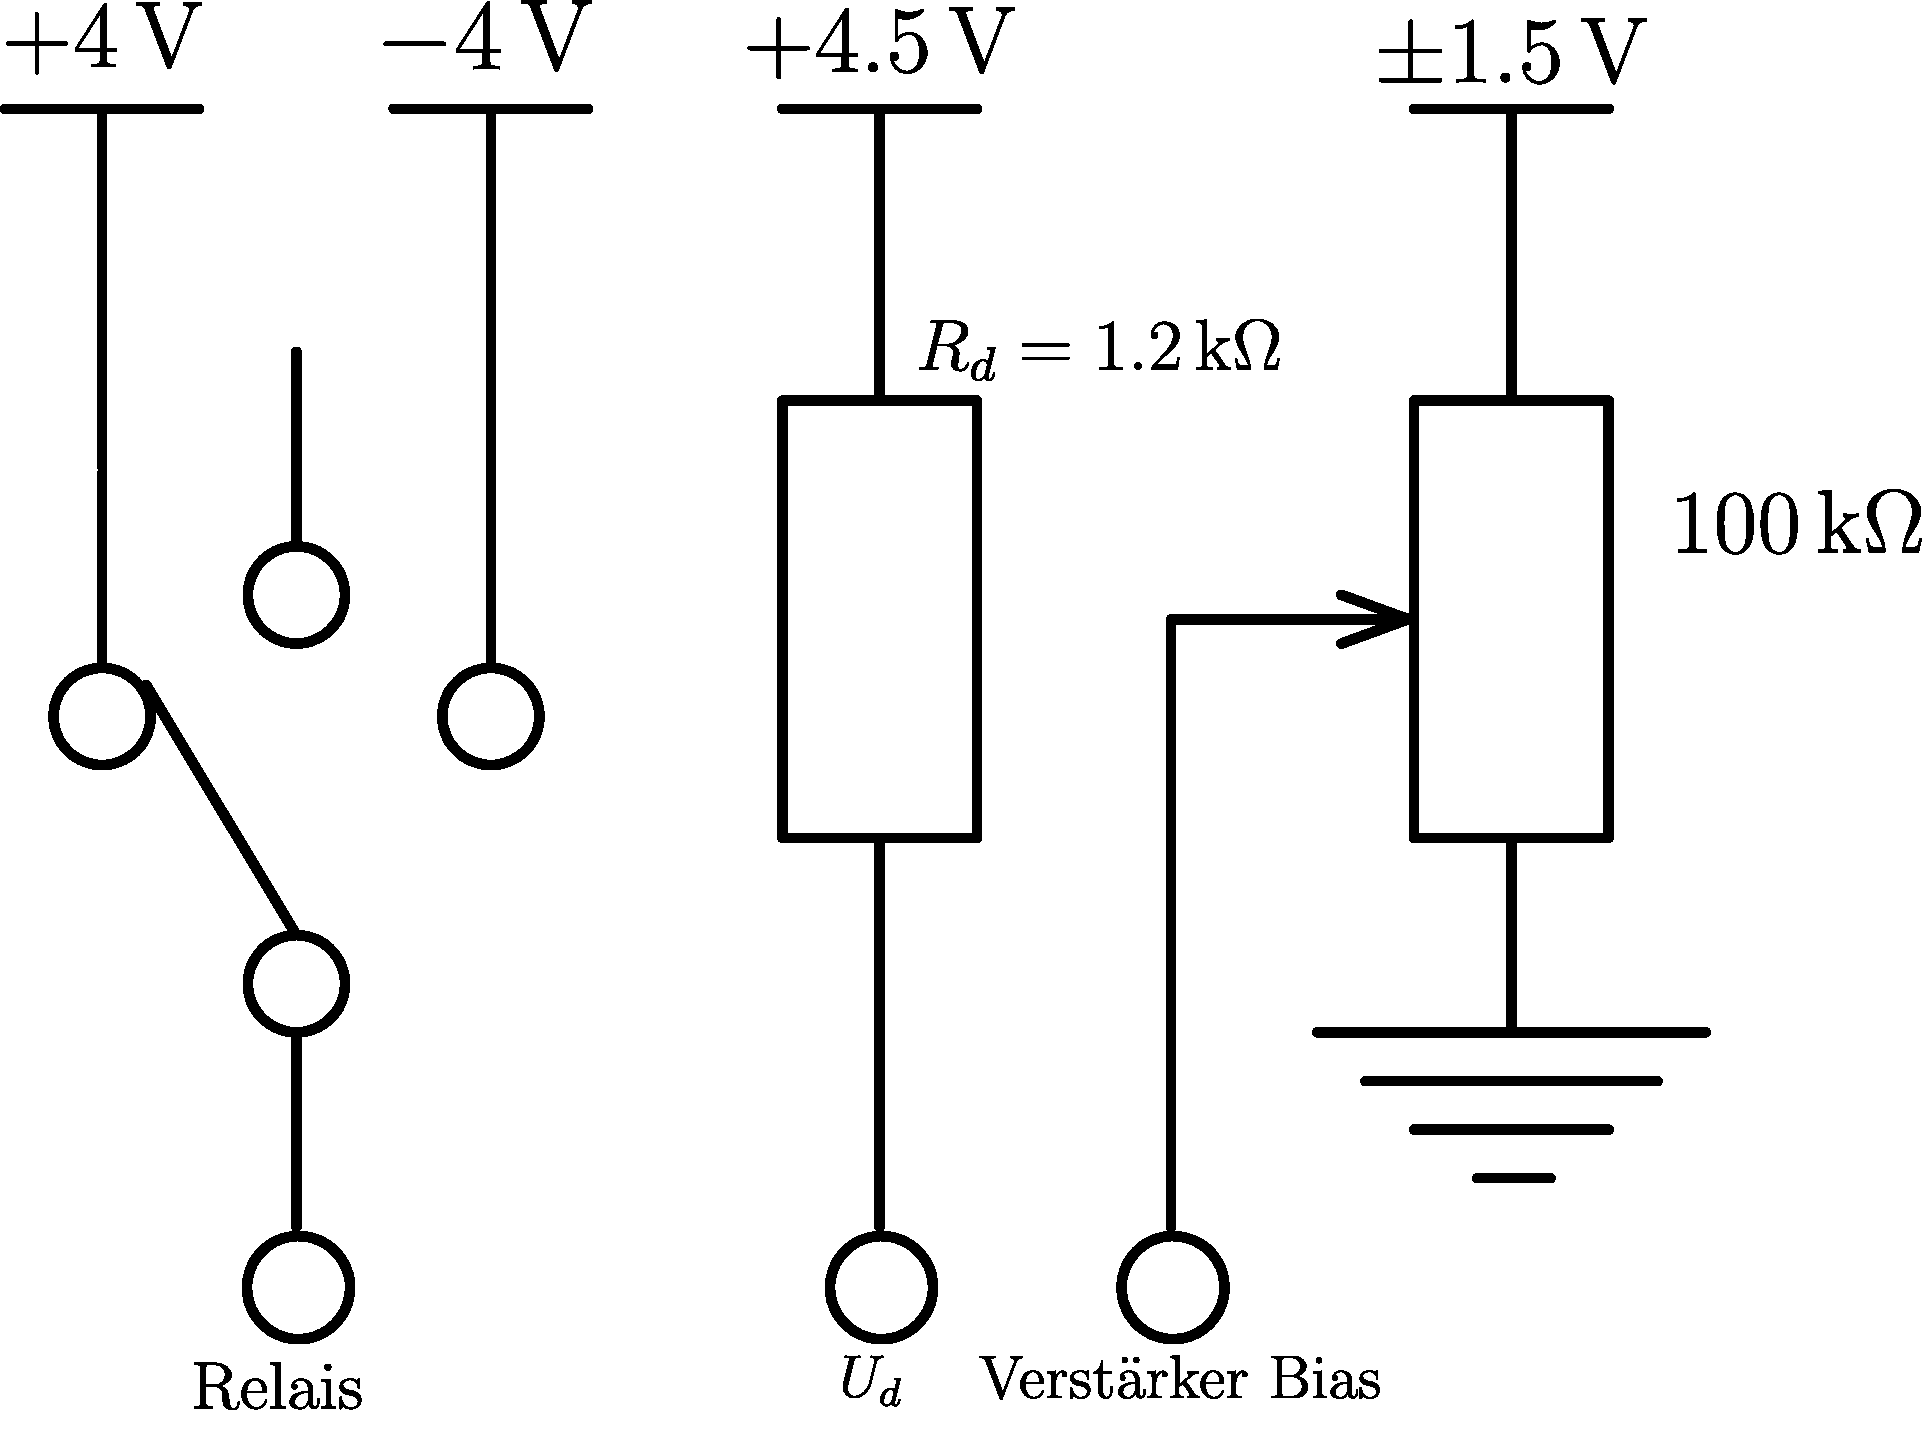
\includegraphics[width=0.5\textwidth]{./fig/Box.pdf}
\vspace{-0.5cm}
\caption{Schaltbild der warmen Elektronik mit einem dreistufigen Schalter zum schalten der Relais, dem Drainwiderstand des Verstärkers und einem Potentiometer um die Biasspannung am Gate des Verstärkers einzustellen.}
\label{fig:WarmeElektronik}
\end{center}
\end{figure}

Um die Handhabung der kalten Elektronik zu vereinfachen gibt es die in Abbildung \ref{fig:WarmeElektronik} gezeigte warme Elektronik.
Mit dem dreistufigen Kippschalter werden die Relais geschaltet.
Die Spannung $U_d$ und der Widerstand $R_d$ ist der Teil des Verstärkers welcher in Abbildung \ref{fig:Amp} außerhalb des Kryostaten ist.
Mit den $\SI{-1.5}{\volt}$ und dem $\SI{100}{\kilo\ohm}$ Potentiometer lässt sich die gewünschte Verstärker Biasspannung eingestellt.
Um das Rauschen zu minimieren und um Rückkopplung über die Spannungsquelle zu vermeiden wird die Drainspannung und die Verstärker Biasspannung mit unabhängigen Batterien versorgt.
Die Spannungen zum Schalten der Relais werden mittels Generator aufgebracht.
Im Warmen befindet sich außerdem ein Oszilloskop mit welchem das in Abbildung \ref{fig:Ausleseelektronik} dargestellte Ausgangssignal aufgenommen wird.
Und ein Signalgenerator mit welchem ein künstliches Signal einer bestimmten Frequenz erzeugt werden kann um die Verstärkung zu bestimmen.
Die Detektor Biasspannung ist für die Funktionsweise der Elektronik unbedeutend und wurde daher auf $\SI{0}{\volt}$ gesetzt.
In Abbildung \ref{fig:ElektronikBilder} sind Bilder der kalten Elektronik (oben Vorder- und Rückansicht) sowie der warmen Elektronik (unten) gezeigt.

Die Kühlung der kalten Elektronik findet mit flüssigem Stickstoff statt.
Dabei wird auf eine aufwendige Temperaturregelung verzichtet weshalb nur das Verhalten bei Raumtemperatur und flüssig Stickstoff Temperatur untersucht wird.
Schließlich befindet sich die kalte Elektronik in einem Faraday-Käfig um sie gegenüber elektromagnetischer Strahlung abzuschirmen.
Allerdings kann elektromagnetische Strahlung trotzdem über die langen Kabel zur Versorgung der Biasspannung und Drainspannung in die Elektronik gelangen.

Um den Aufbau so authentisch wie möglich zu gestalten in der kalten Elektronik ein \textit{dummy detector} eingebaut.
Dieser entspricht einer Kapazität zu Ground der selben Größe wie die Detektorkapazität $C_d$.

Die Daten der kalten Elektronik werden für verschiedenen handelsübliche HEMTs aufgenommen.

\begin{figure}[!t]
\begin{center}
\includegraphics[width=\textwidth]{./fig/ElektronikBilder.pdf}
\vspace{-0.5cm}
\caption{Bilder der warmen und kalten Elektronik.
Oben rechts: Rückseite der kalten Elektronik. Oben link: Vorderseite der kalten Elektronik.
Unten: Warme Elektronik im Gehäuse.}
\label{fig:ElektronikBilder}
\end{center}
\end{figure}
